\begin{frame}{3. ¿Puede una recta aprender el cuadrado?}
    \begin{columns}[c]
        \begin{column}{0.26\textwidth}
            \centering\small
            \textbf{Función cuadrática}\par\medskip
            \begin{tabular}{rr}
                \toprule
                Entrada $x$ & Salida $y$\\
                \midrule
                $-2$ & $4$\\
                $-1$ & $1$\\
                $0$ & $0$\\
                $1$ & $1$\\
                $2$ & $4$\\
                \bottomrule
            \end{tabular}
            \par\medskip $y=x^2$\par\smallskip
            \scriptsize Muestra de los 21 pares de entrenamiento.
        \end{column}
        \begin{column}{0.70\textwidth}
            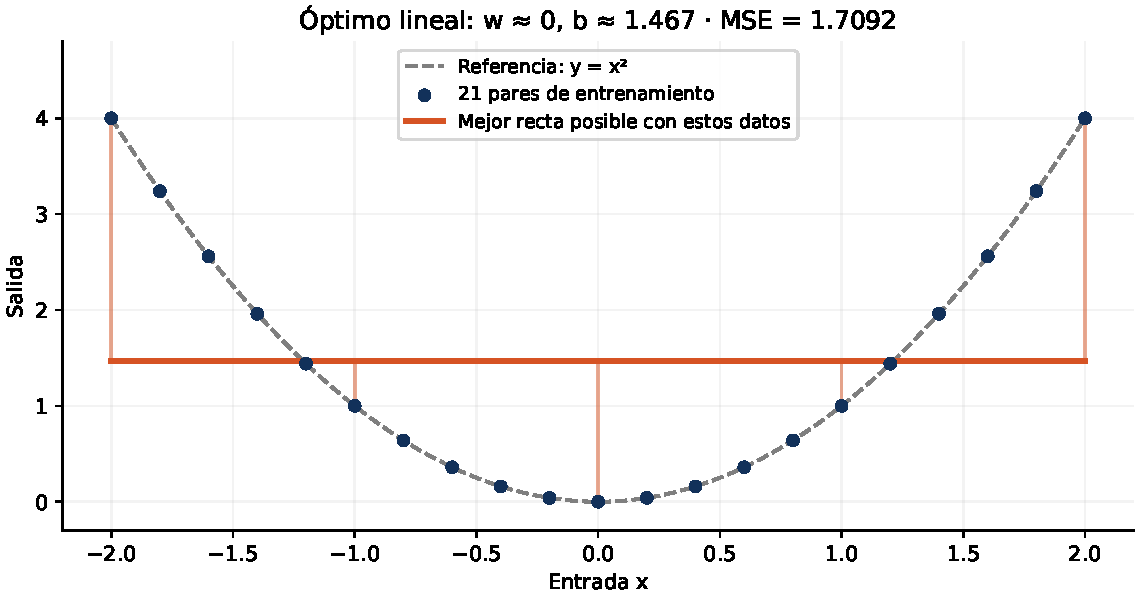
\includegraphics[width=\linewidth,height=4.3cm,keepaspectratio]{limite_lineal_cuadrado.pdf}
        \end{column}
    \end{columns}
    \medskip
    \begin{caja}[orangebox]
        \textbf{Ajustar mejor los parámetros no cambia la forma del modelo.}\par\smallskip
        $\hat y=wx+b$ sigue siendo una recta; no reproduce la curvatura de $x^2$.
    \end{caja}
    \smallskip\small Necesitamos ampliar la familia de funciones: el siguiente ejemplo incorpora activaciones no lineales.
    \note{La recta naranja es el mejor ajuste por mínimos cuadrados a los 21 pares, no una mala inicialización. Por simetría, su pendiente es cero y el sesgo es el promedio de los cuadrados. Incluso el óptimo deja residuos: añadir épocas no elimina ese límite. Una recta puede aproximar localmente una curva, pero no reproducir x al cuadrado en todo este intervalo. Se considera x como única característica: añadir x al cuadrado como característica sería cambiar la representación. La siguiente diapositiva conserva la simulación de la red no lineal.}
\end{frame}
